%! Author = TiagoRG
%! GitHub = https://github.com/TiagoRG

\chapter{Detalhes Experimentais Relevantes}
\label{ch:detalhes-experimentais-relevantes}
{
%%%
% Conteúdo da introdução aqui
\section{Material}
\label{subsec:detalhes-experimentais-relevantes-material}

\begin{enumerate}
    \item Voltímetro
    \item Amperímetro
    \item Fonte de tensão de $15~V$
    \item Resistência de $10~\Omega$
    \item Reóstato de $330~\Omega$
    \item Sonda de efeito de Hall
    \item Solenoide
    \item Bobines de Helmholtz
\end{enumerate}

\begin{figure}[H]
    \centering
    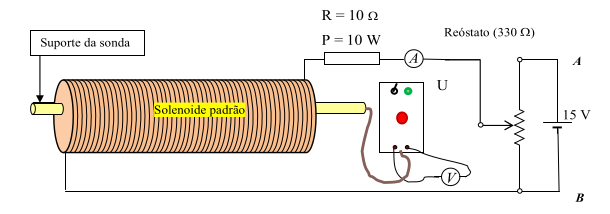
\includegraphics[width=1\linewidth]{images/esquema-montagem-experimental.png}
    \caption{Montagem experimental}
    \label{fig:detalhes-experimentais-relevantes-montagem-experimental}
\end{figure}

\pagebreak

\section{Parte A}
\label{sec:detalhes-experimentais-relevantes-parte1}

Esta primeira parte do trabalho foi realizada com o objetivo de calibrar a sonda de efeito de Hall, obtendo assim a sua constante de calibração ($C_c$), a ser usada na segunda parte do trabalho.

\subsection{Procedimento}
\label{subsec:detalhes-experimentais-relevantes-parte1-procedimento}

\begin{enumerate}
    \item Liga-se a sonda ao voltímetro e regula-se o potenciómetro da sonda para que o voltímetro indique $0~V$ quando não está sujeita a um campo magnético.
    \item Monta-se agora o resto do circuito, como na figura \ref{fig:detalhes-experimentais-relevantes-montagem-experimental}.
    \item Regista-se o valor $\frac{N}{l}$, que é o número de espiras por unidade de comprimento do solenoide.
    \item Coloca-se a sonda no interior do solenoide, procurando o ponto onde a aproximação utilizada de solenoide infinito.
    \item Ajusta-se o reóstato de modo a obter 10 valores de corrente $I_S$ diferentes, registando-se os diferentes valores da tensão $V_H$ para cada valor da corrente.
\end{enumerate}

\section{Parte B}
\label{sec:detalhes-experimentais-relevantes-parte2}

\subsection{Procedimento}
\label{subsec:detalhes-experimentais-relevantes-parte2-procedimento}

\begin{enumerate}
    \item Colocam-se as bobines na configuração de Helmholtz, com uma distância entre elas igual ao seu raio.
    \item Registam-se os dados das bobines, nomeadamente o raio e posição de cada uma.
    \item Monta-se agora o resto do circuito, como na figura \ref{fig:detalhes-experimentais-relevantes-montagem-experimental} apenas substituindo o solenoide por uma das bobines.
    \item Ajusta-se o reóstato de modo a ter $I=0.50A$ que será constante durante toda a experiência.
    \item Mede-se o campo magnético criado pela bobine ao longo do seu eixo, de centímetro a centímetro, registando cada par de valores: posição, tensão de Hall $(V_H)$.
    \item Repetem-se os passos 3, 4 e 5, mas agora para a segunda bobine (usando as mesmas posições usadas anteriormente).
    \item Ligam-se agora ambas as bobines, em série, e mais uma vez registam-se os valores da tensão de Hall para as mesmas posições utilizadas anteriormente.
\end{enumerate}

\pagebreak

%%%
}
